\documentclass[lettersize,journal]{IEEEtran}
\usepackage{amsmath,amsfonts}
\usepackage{algorithmic}
\usepackage{algorithm}
\usepackage{array}
\usepackage[caption=false,font=normalsize,labelfont=sf,textfont=sf]{subfig}
\usepackage{textcomp}
\usepackage{stfloats}
\usepackage{url}
\usepackage{verbatim}
\usepackage{graphicx}
\usepackage{cite}
\usepackage{tikz}
\usetikzlibrary{positioning, calc, shapes, arrows, fit}
\usepackage{circuitikz}
\hyphenation{op-tical net-works semi-conduc-tor IEEE-Xplore}
\graphicspath{{images/}}
% updated with editorial comments 8/9/2021

\begin{document}

\title{Lab 3 -- Generating and Measuring Waveforms}

\author{Benjamin Sage\\Lab Partners: Marc Huerta, Devorah Simon}

% The paper headers
\markboth{EE 133: Analog Communications Design Laboratory, February~2022}%
{Shell \MakeLowercase{\textit{et al.}}: A Sample Article Using IEEEtran.cls for IEEE Journals}

% \IEEEpubid{0000--0000/00\$00.00~\copyright~2021 IEEE}
% Remember, if you use this you must call \IEEEpubidadjcol in the second
% column for its text to clear the IEEEpubid mark.

\maketitle

\begin{abstract}
A MOSFET mixer was built and analyzed using a spectrum analyzer. Several important uses and properties of this mixer emerged during the study.
\end{abstract}

% \begin{IEEEkeywords}
% Article submission, IEEE, IEEEtran, journal, \LaTeX, paper, template, typesetting.
% \end{IEEEkeywords}

\section{Introduction}
\IEEEPARstart{A}{} mixer is a three-port electronic device that modulates a waveform's frequency without changing the amplitude or phase.

\begin{figure}[h]
\centering
\begin{circuitikz}
\draw node[mixer] (mix) {};
\draw[->] (mix) -- ++(2, 0) node[midway, label=IF] {};
\draw[<-] (mix) -- ++(-2, 0) node[midway, label=RF] {};
\draw[<-] (mix) -- ++(0, -2) node[midway, label=right:LO] {};
\end{circuitikz}
\caption{An Ideal Mixer}
\end{figure}

The mixer has two input ports. LO, or local oscillator, gets added to or subtracted from RF to generate new frequencies, which are sent to the output IF, or intermediate frequency.

The mixer built in this lab is called a double-balanced FET ring mixer. It utilizes a ring of four MOSFET transistors to mix the LO with the RF. A schematic can be seen in Fig. 2.

\begin{figure}[!t]
\centering
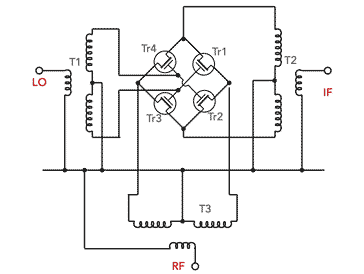
\includegraphics[width=2.5in]{circuit}
\caption{Double-balanced FET Mixer}
\label{fig_1}
\end{figure}

\section{Experimental Setup}

The setup for this experiment consisted of 2 parts:
\begin{enumerate}
    \item {\bf{Wave Generator}} Used to produce both the local oscillator (LO) and radio frequency (RF) signals.
    \item {\bf{Spectrum Analyzer}} Used to measure the intermediate frequency (IF) output.
\end{enumerate}

\section{Measurements and Results}

To begin, we mixed a $2 \, \text{MHz}$ radio frequency signal with a $10 \, \text{MHz}$ local oscillator frequency. As shown in {\bf{Table 1}} and Fig. 3, we achieved the expected result of sums and differences of the frequencies in the intermedite frequency.

Interstingly, we also get harmonic frequencies around $28$ and $32$ MHz.

\begin{table}
\renewcommand{\arraystretch}{2.2}
\begin{center}
\caption{Mixer Port Frequencies}
\label{tab1}
\begin{tabular}{c c}
\hline
\bfseries Port & \bfseries Frequency\\
\hline
RF & $2 \, \text{MHz}$\\
\hline
LO & $10 \, \text{MHz}$\\ 
\hline
IF & $10 \pm 2 \, \text{MHz}$\\
\hline
\end{tabular}
\end{center}
\end{table}

\begin{figure}[!t]
\centering
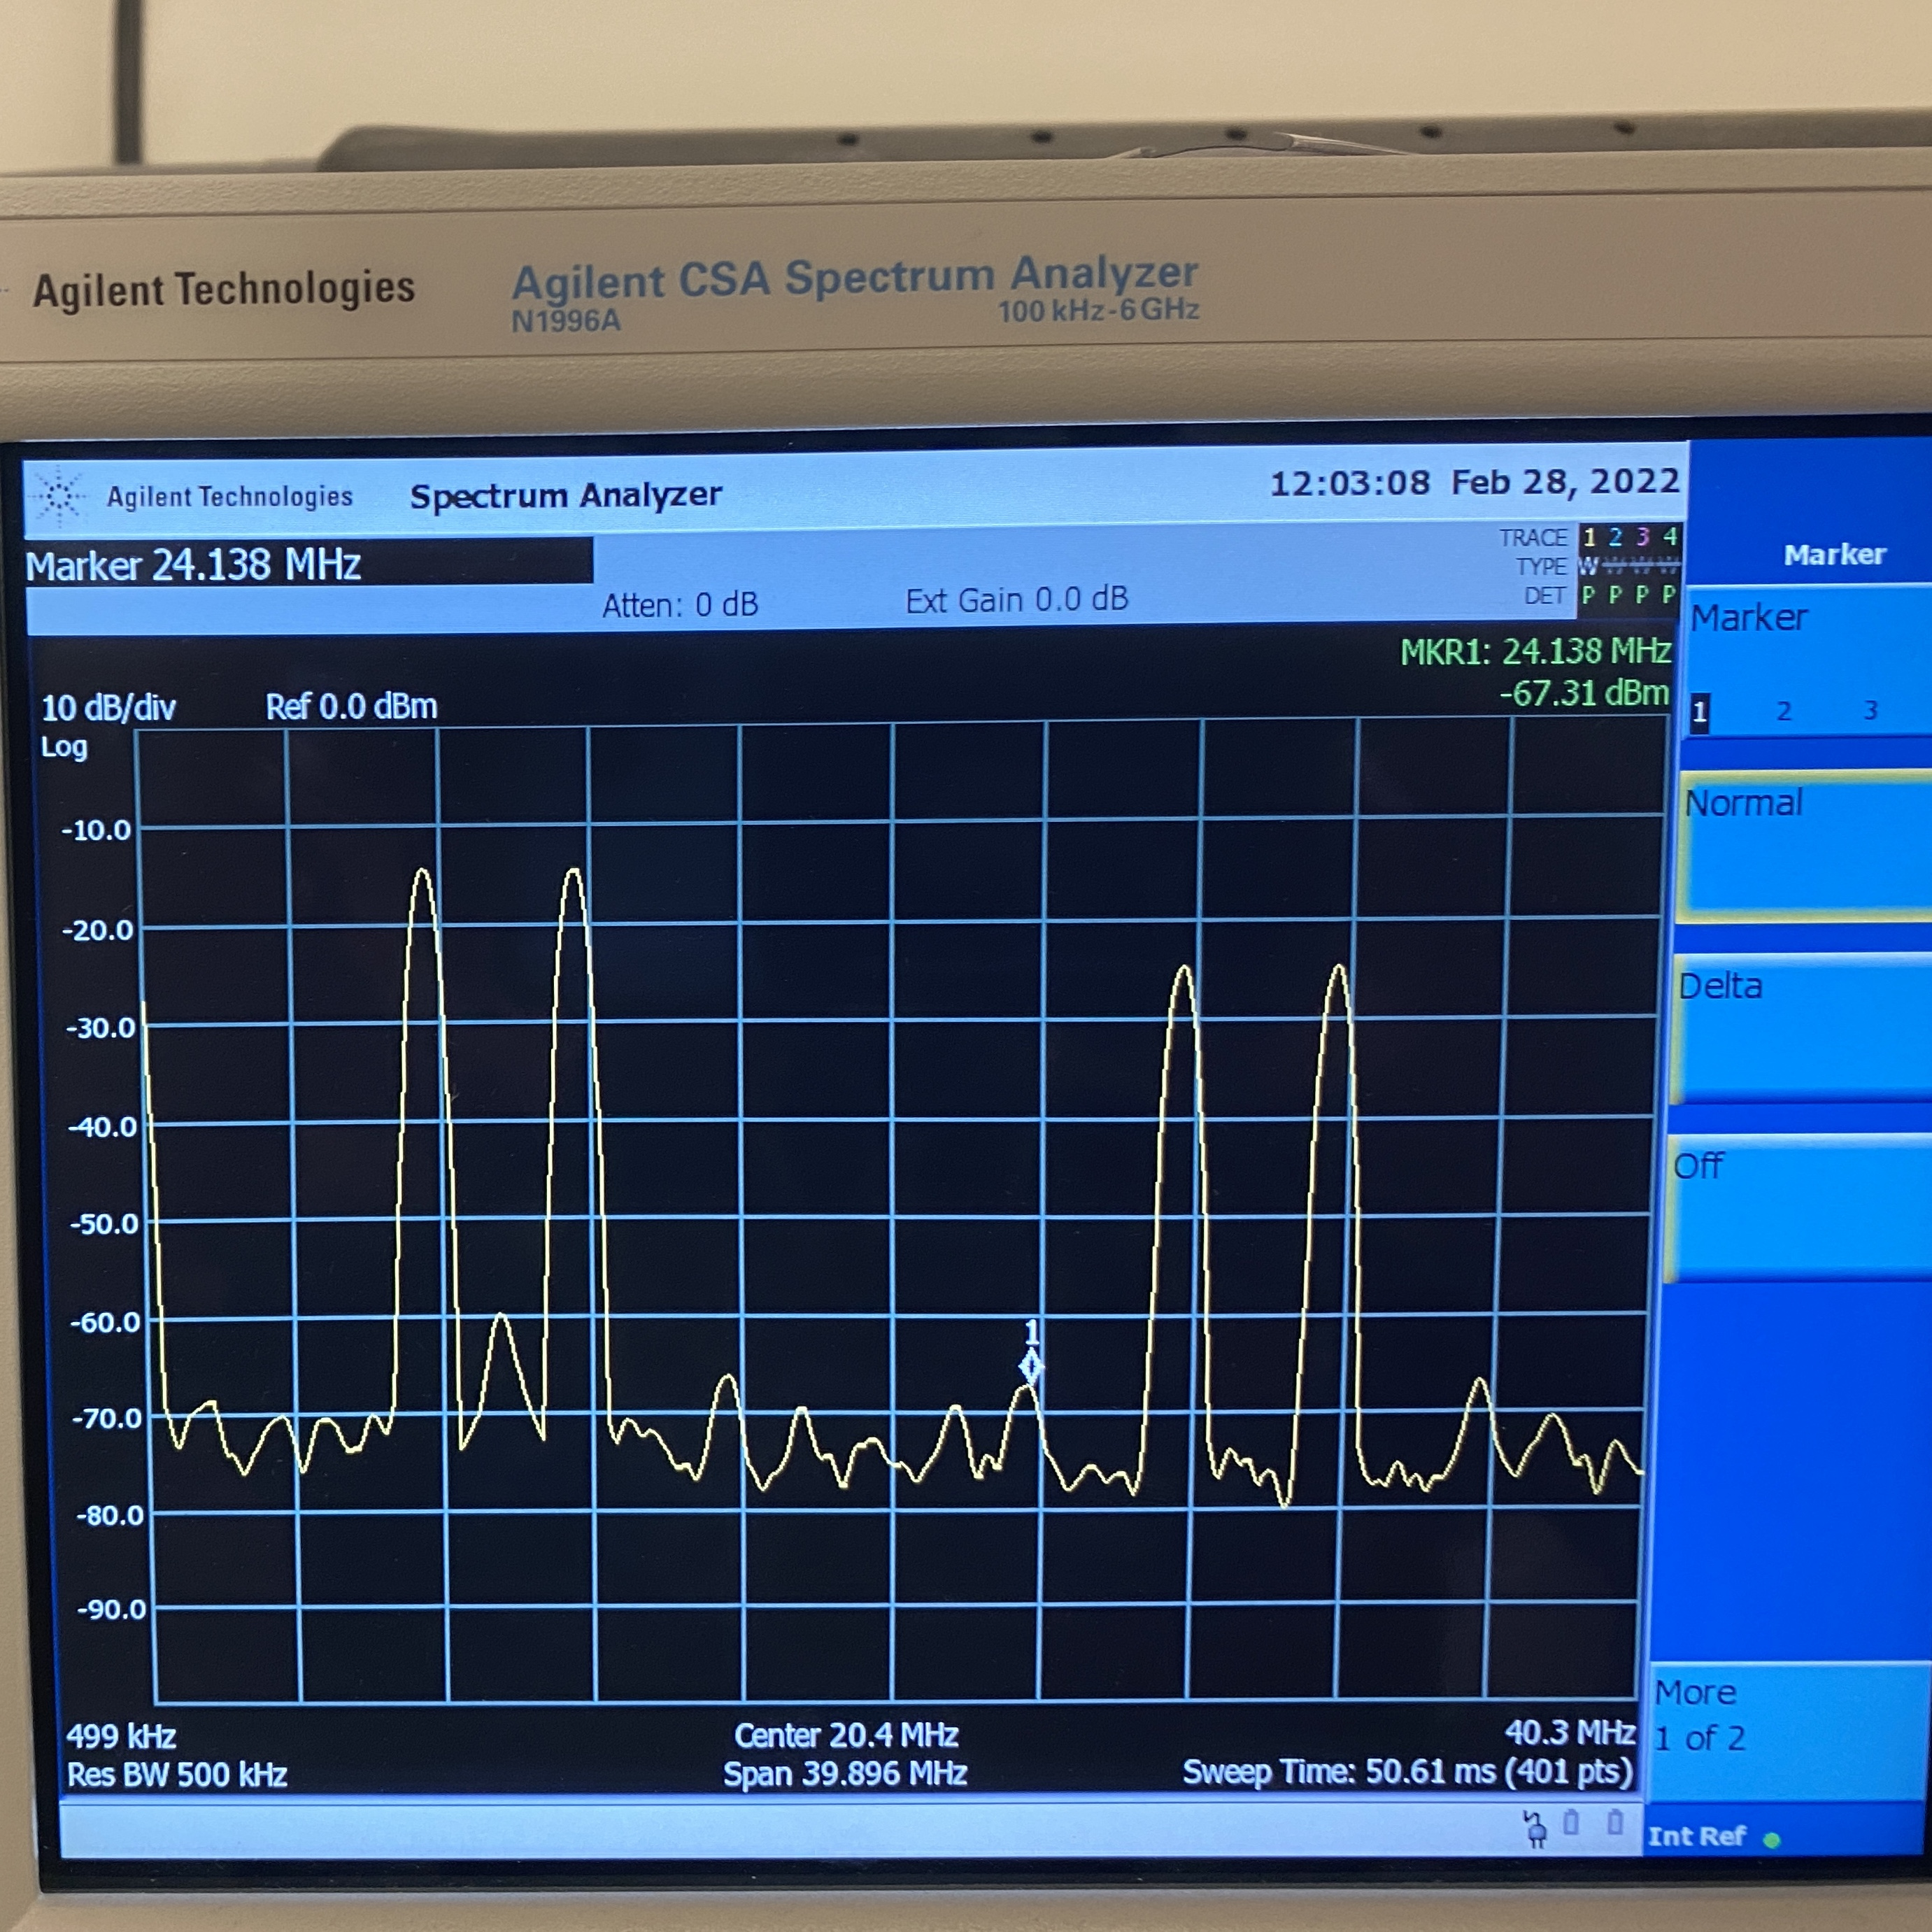
\includegraphics[width=2.3in]{first}
\caption{Intermediate frequency spectrum, with peaks around 8 and 12 MHz.}
\label{fig_1}
\end{figure}

\subsection{Changing the Amplitude of RF}

We can modulate the amplitude of the radio frequency signal to see if it has an effect on output. See the results in Fig. 4. A larger amplitude results both in greater gain as well as greater noise.

\begin{figure*}[!t]
\centering
\subfloat[]{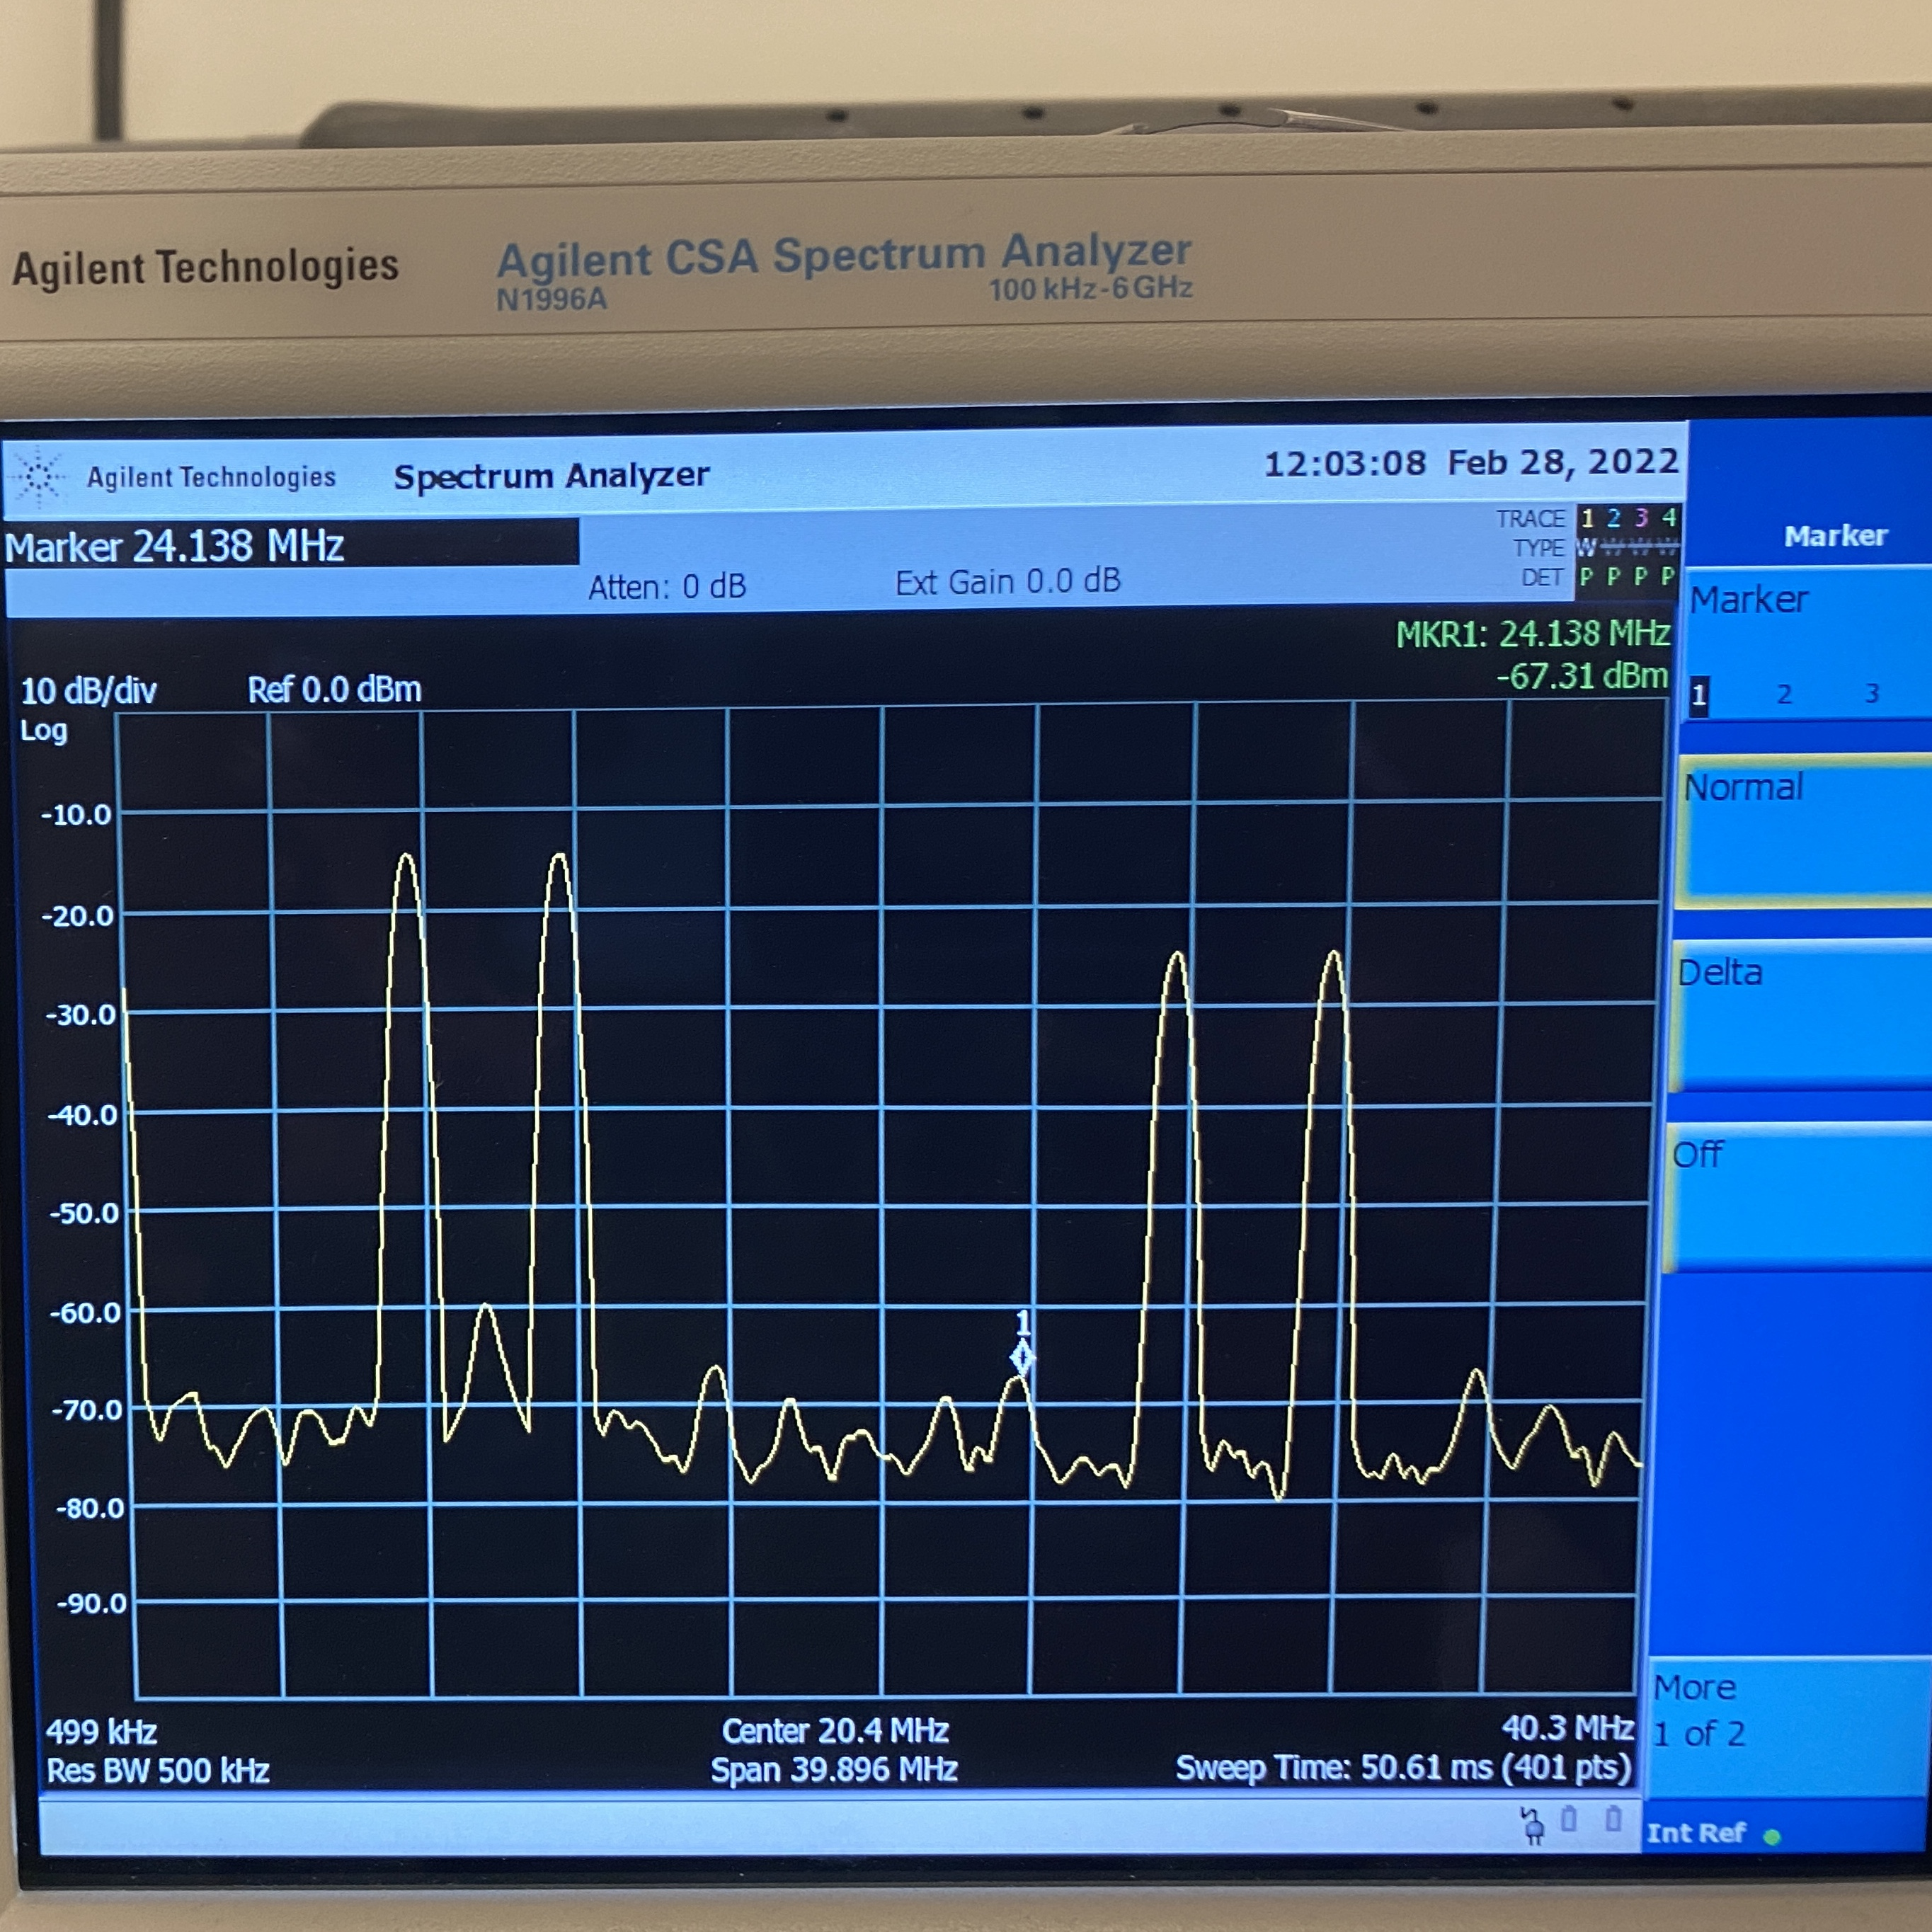
\includegraphics[width=2.5in]{second}%
\label{fig_first_case}}
\hfil
\subfloat[]{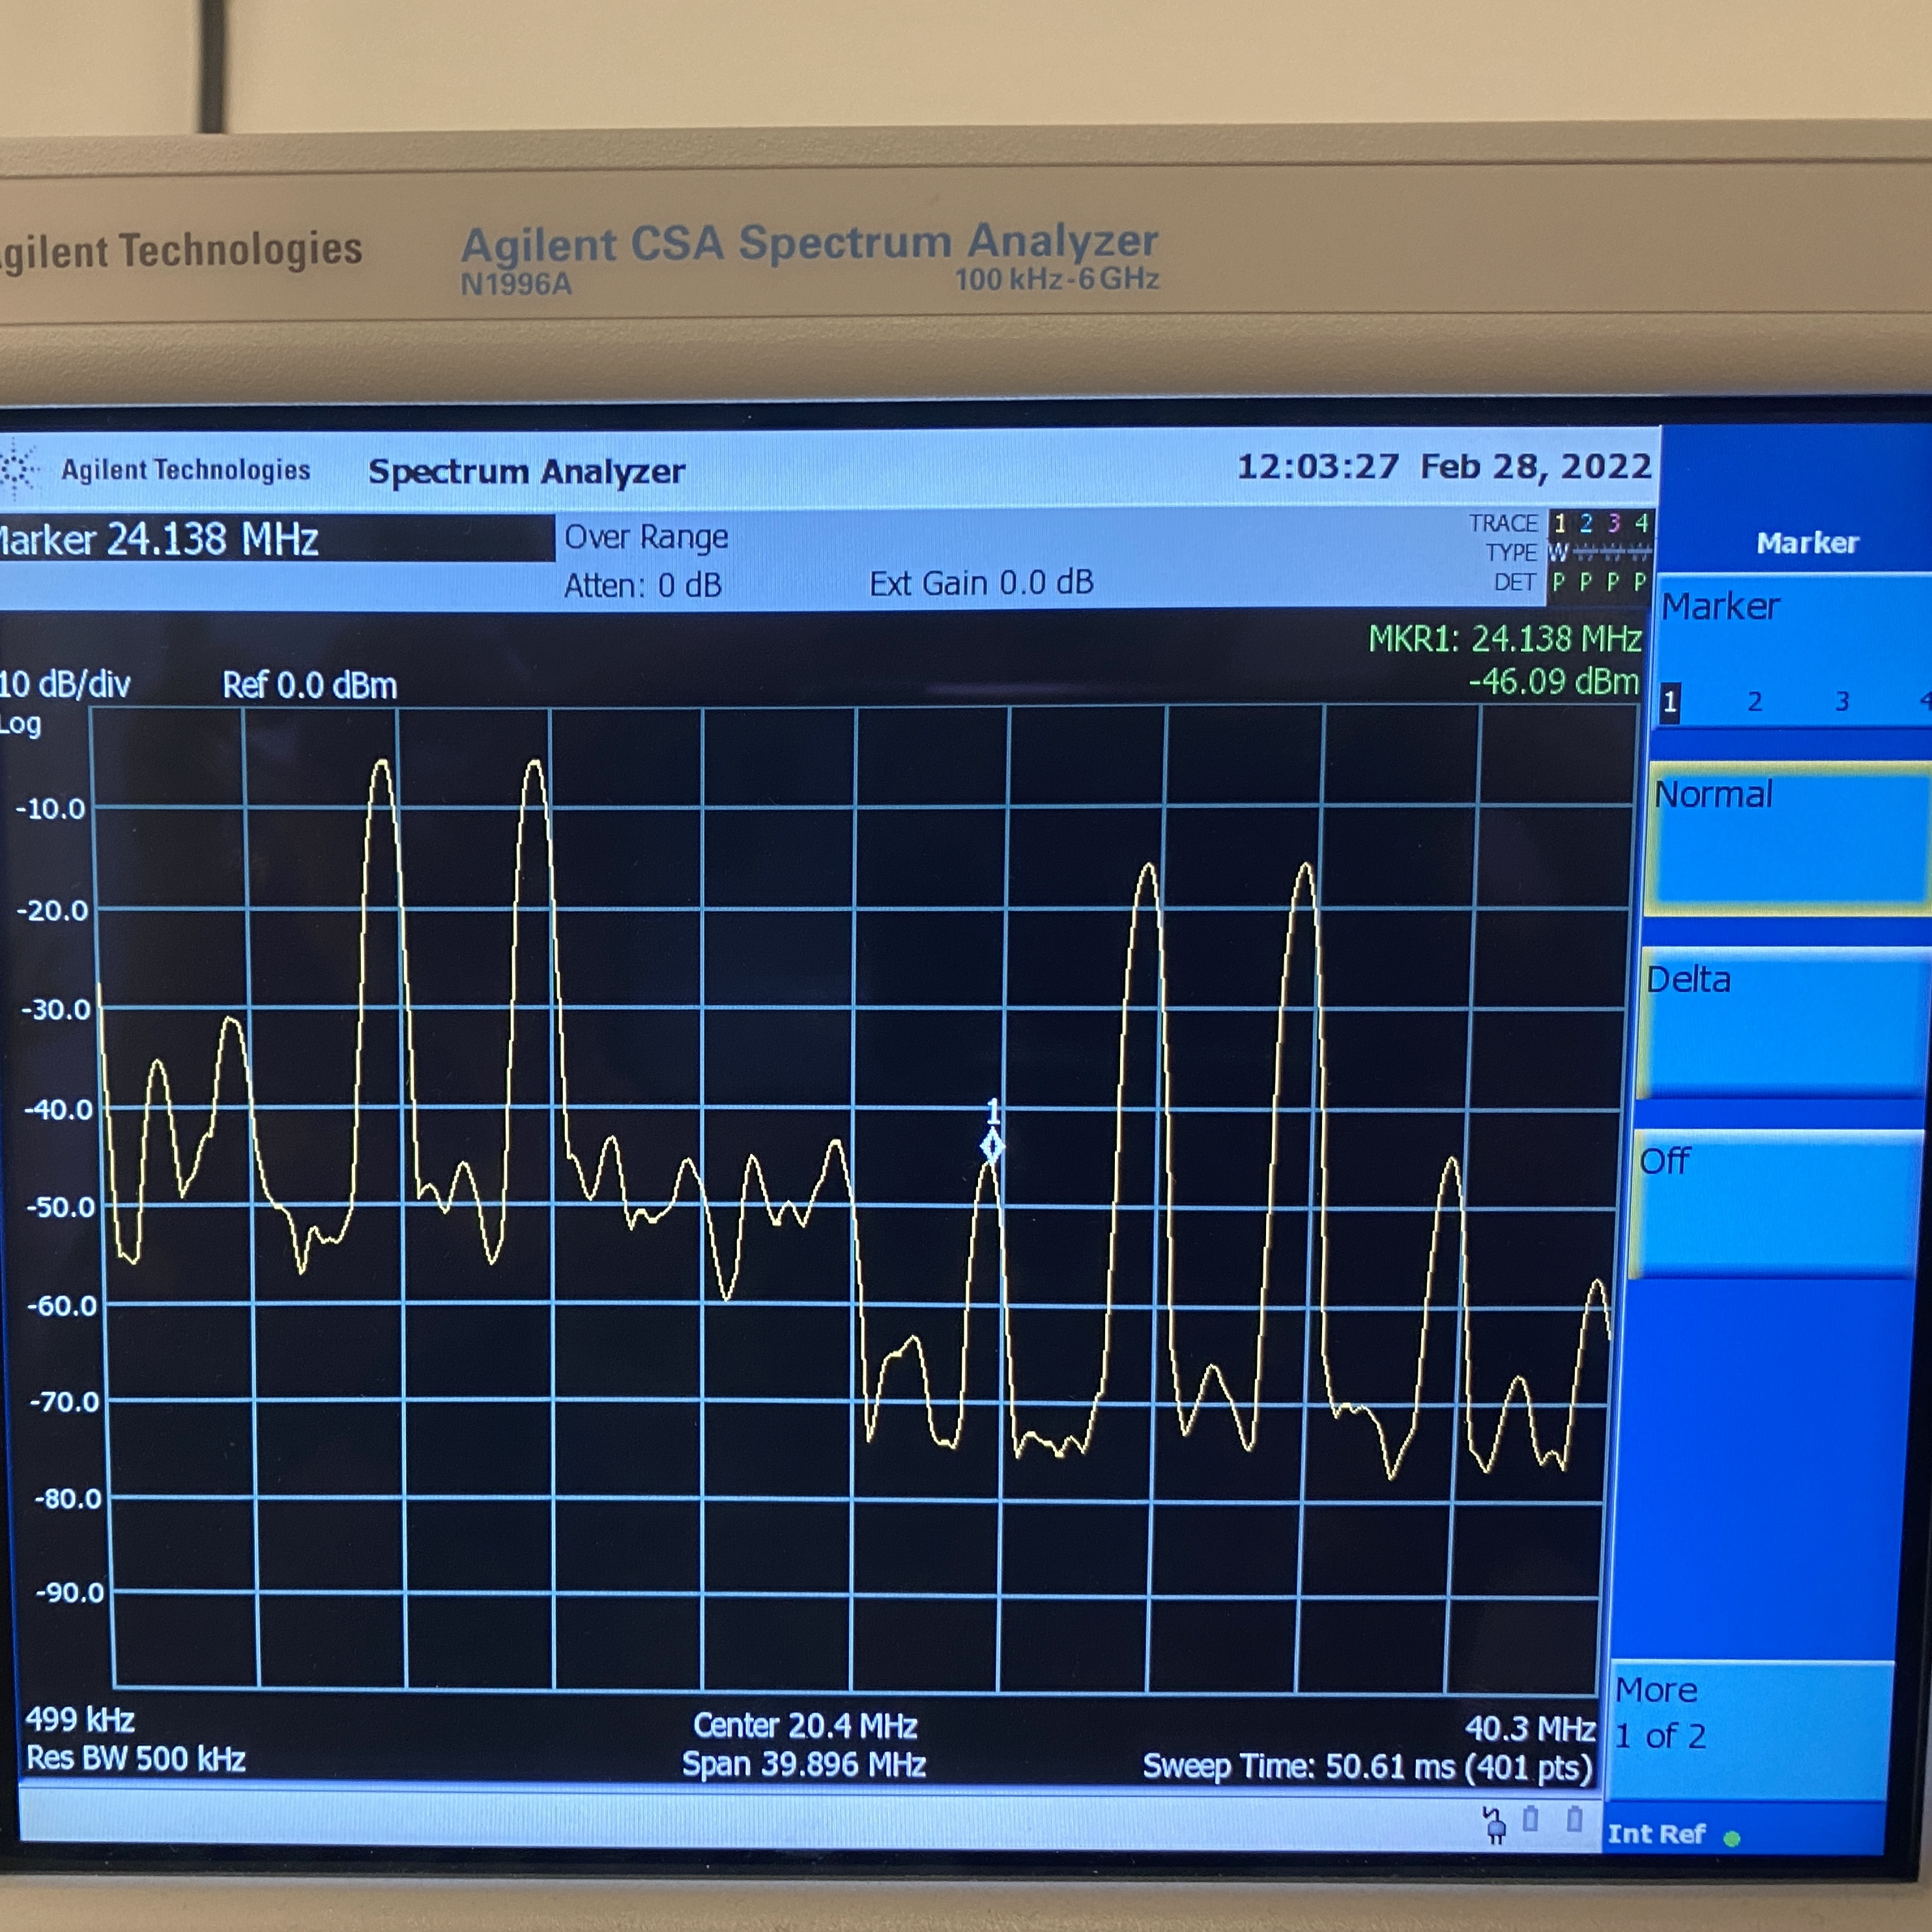
\includegraphics[width=2.5in]{third}%
\label{fig_third_case}}
\caption{Increasing the amplitude of RF increases the gain as well as the noise. In (a), the amplitude is $0.5\,\text{V}_{pp}$, while in (b), it is $1.5\,\text{V}_{pp}$}
\label{fig_si}
\end{figure*}

\subsection{Changing the Amplitude of LO}

We can also modulate the amplitude of the local oscillator signal to see if it has an effect on output. See the results in Fig. 5. A larger amplitude again results both in greater gain as well as greater noise.

\begin{figure*}[!t]
\centering
\subfloat[]{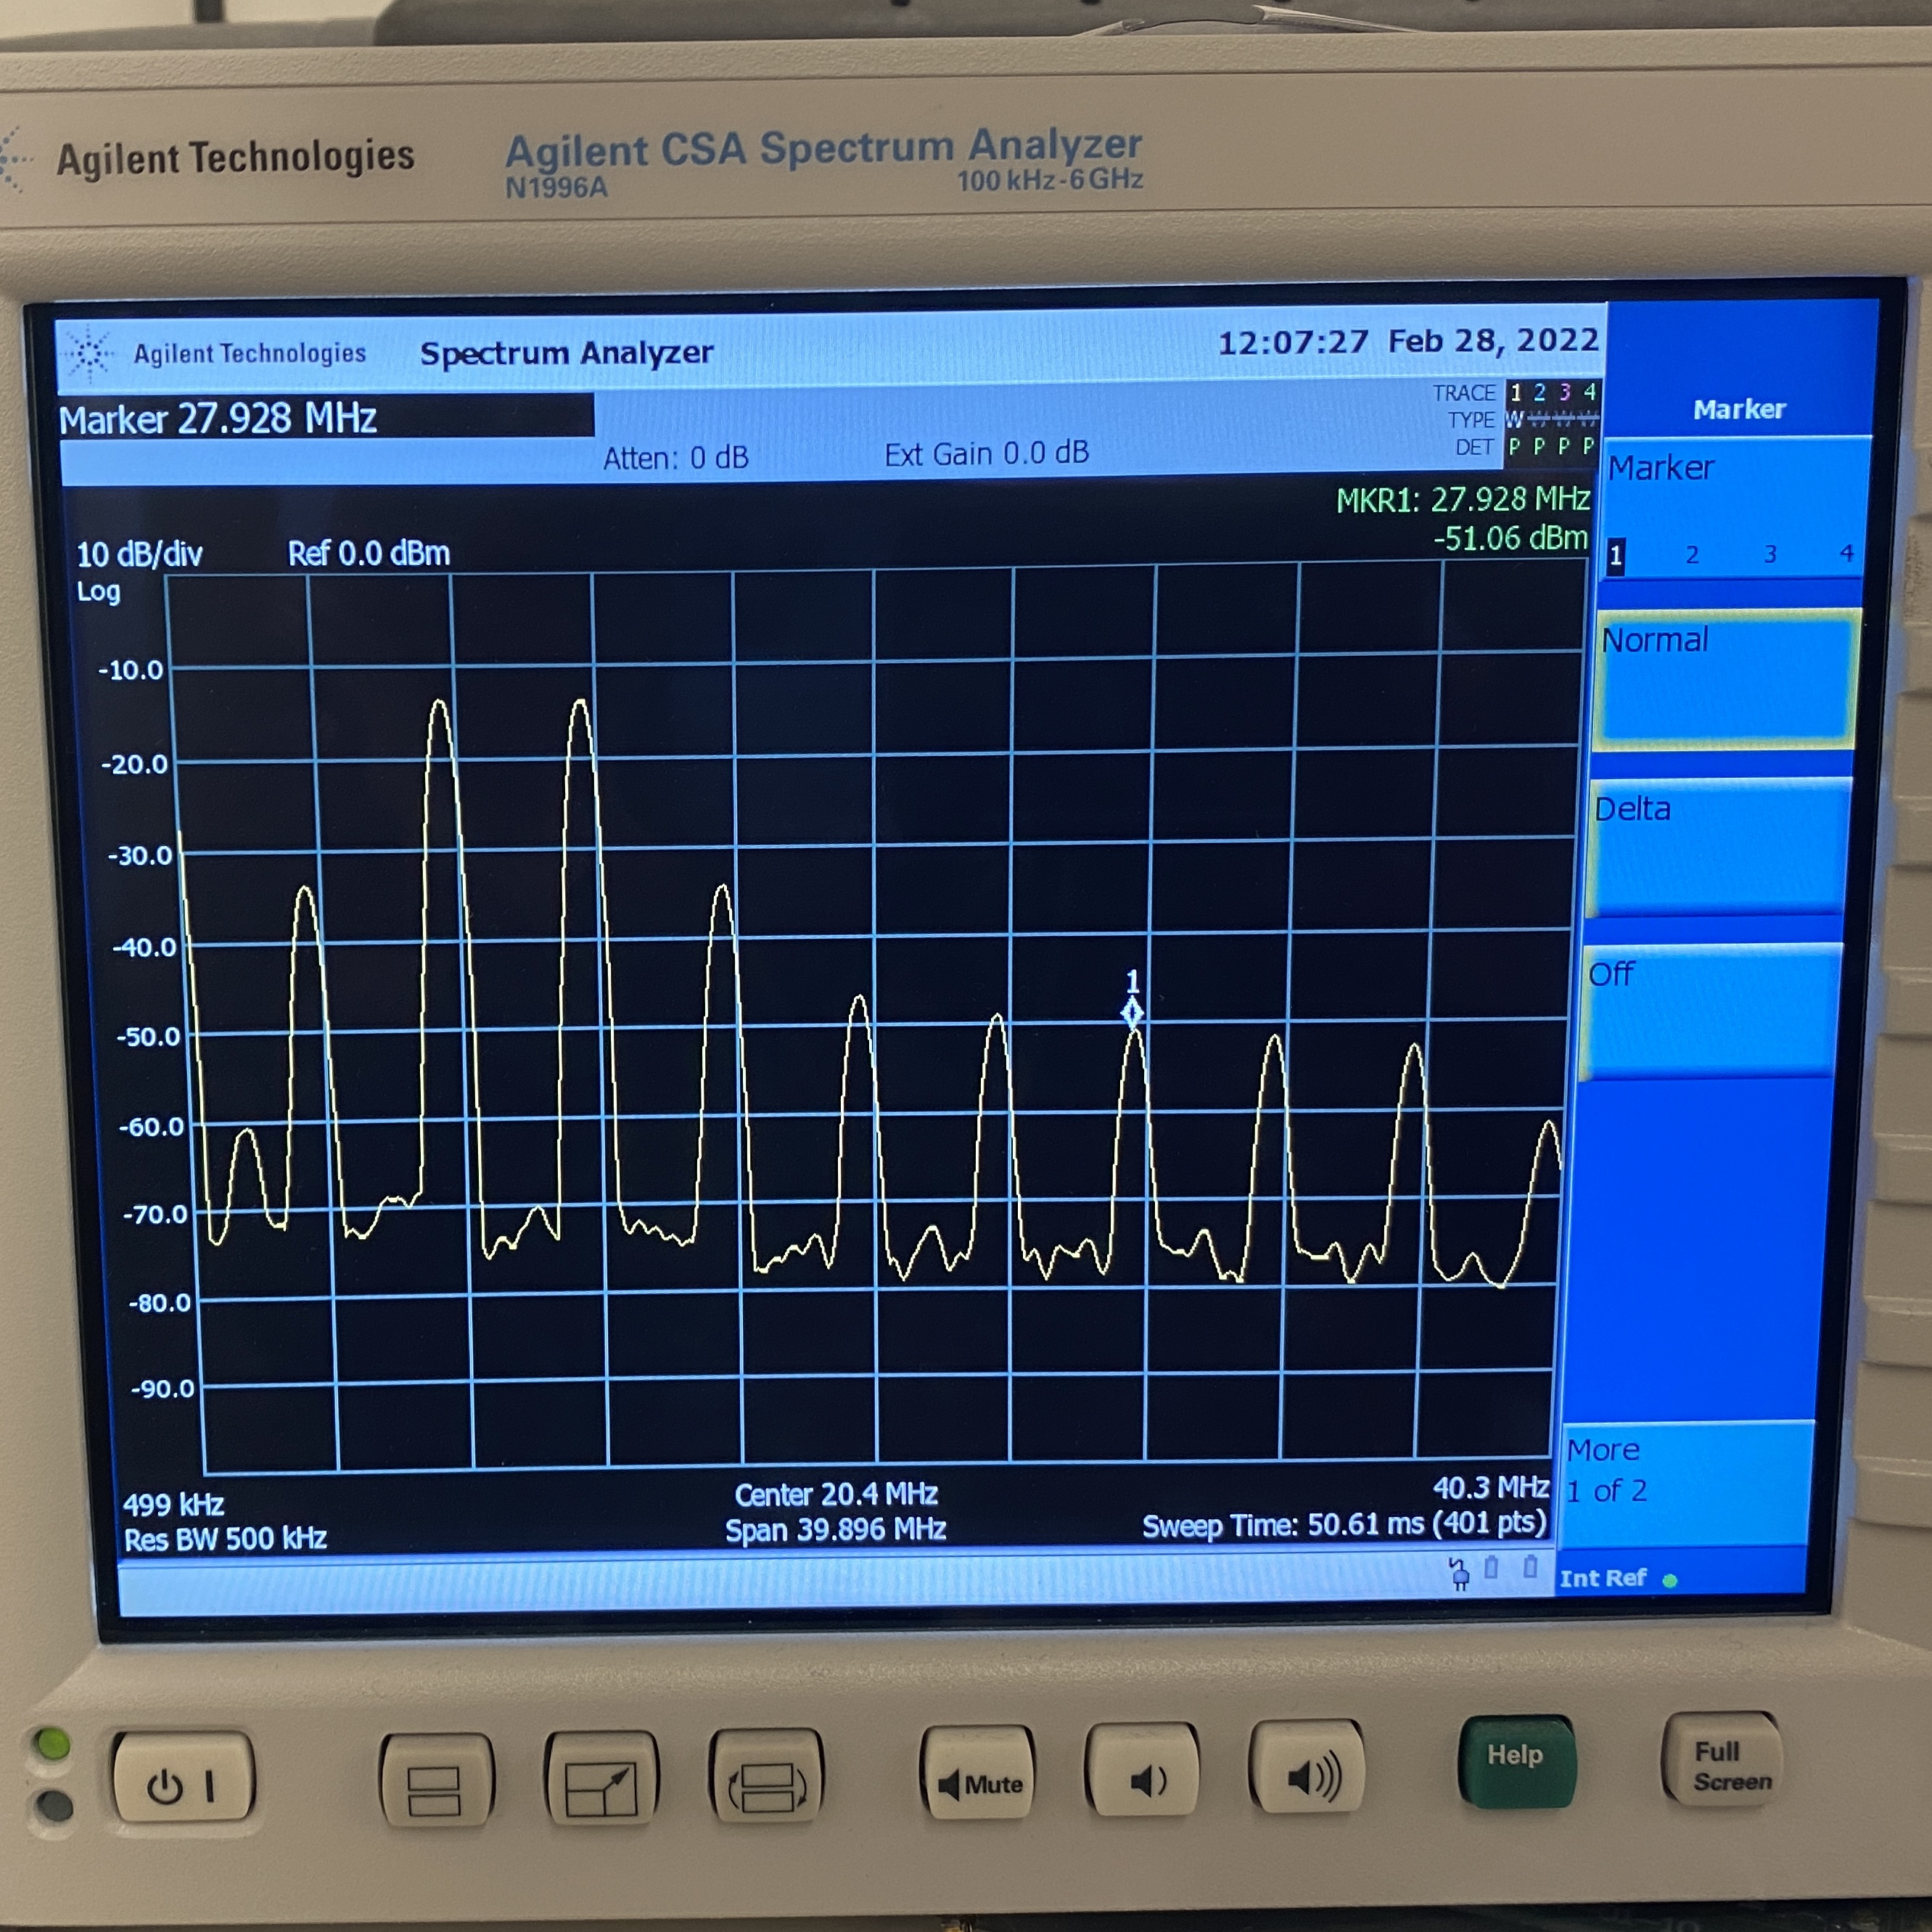
\includegraphics[width=2.5in]{fourth}%
\label{fig_first_case}}
\hfil
\subfloat[]{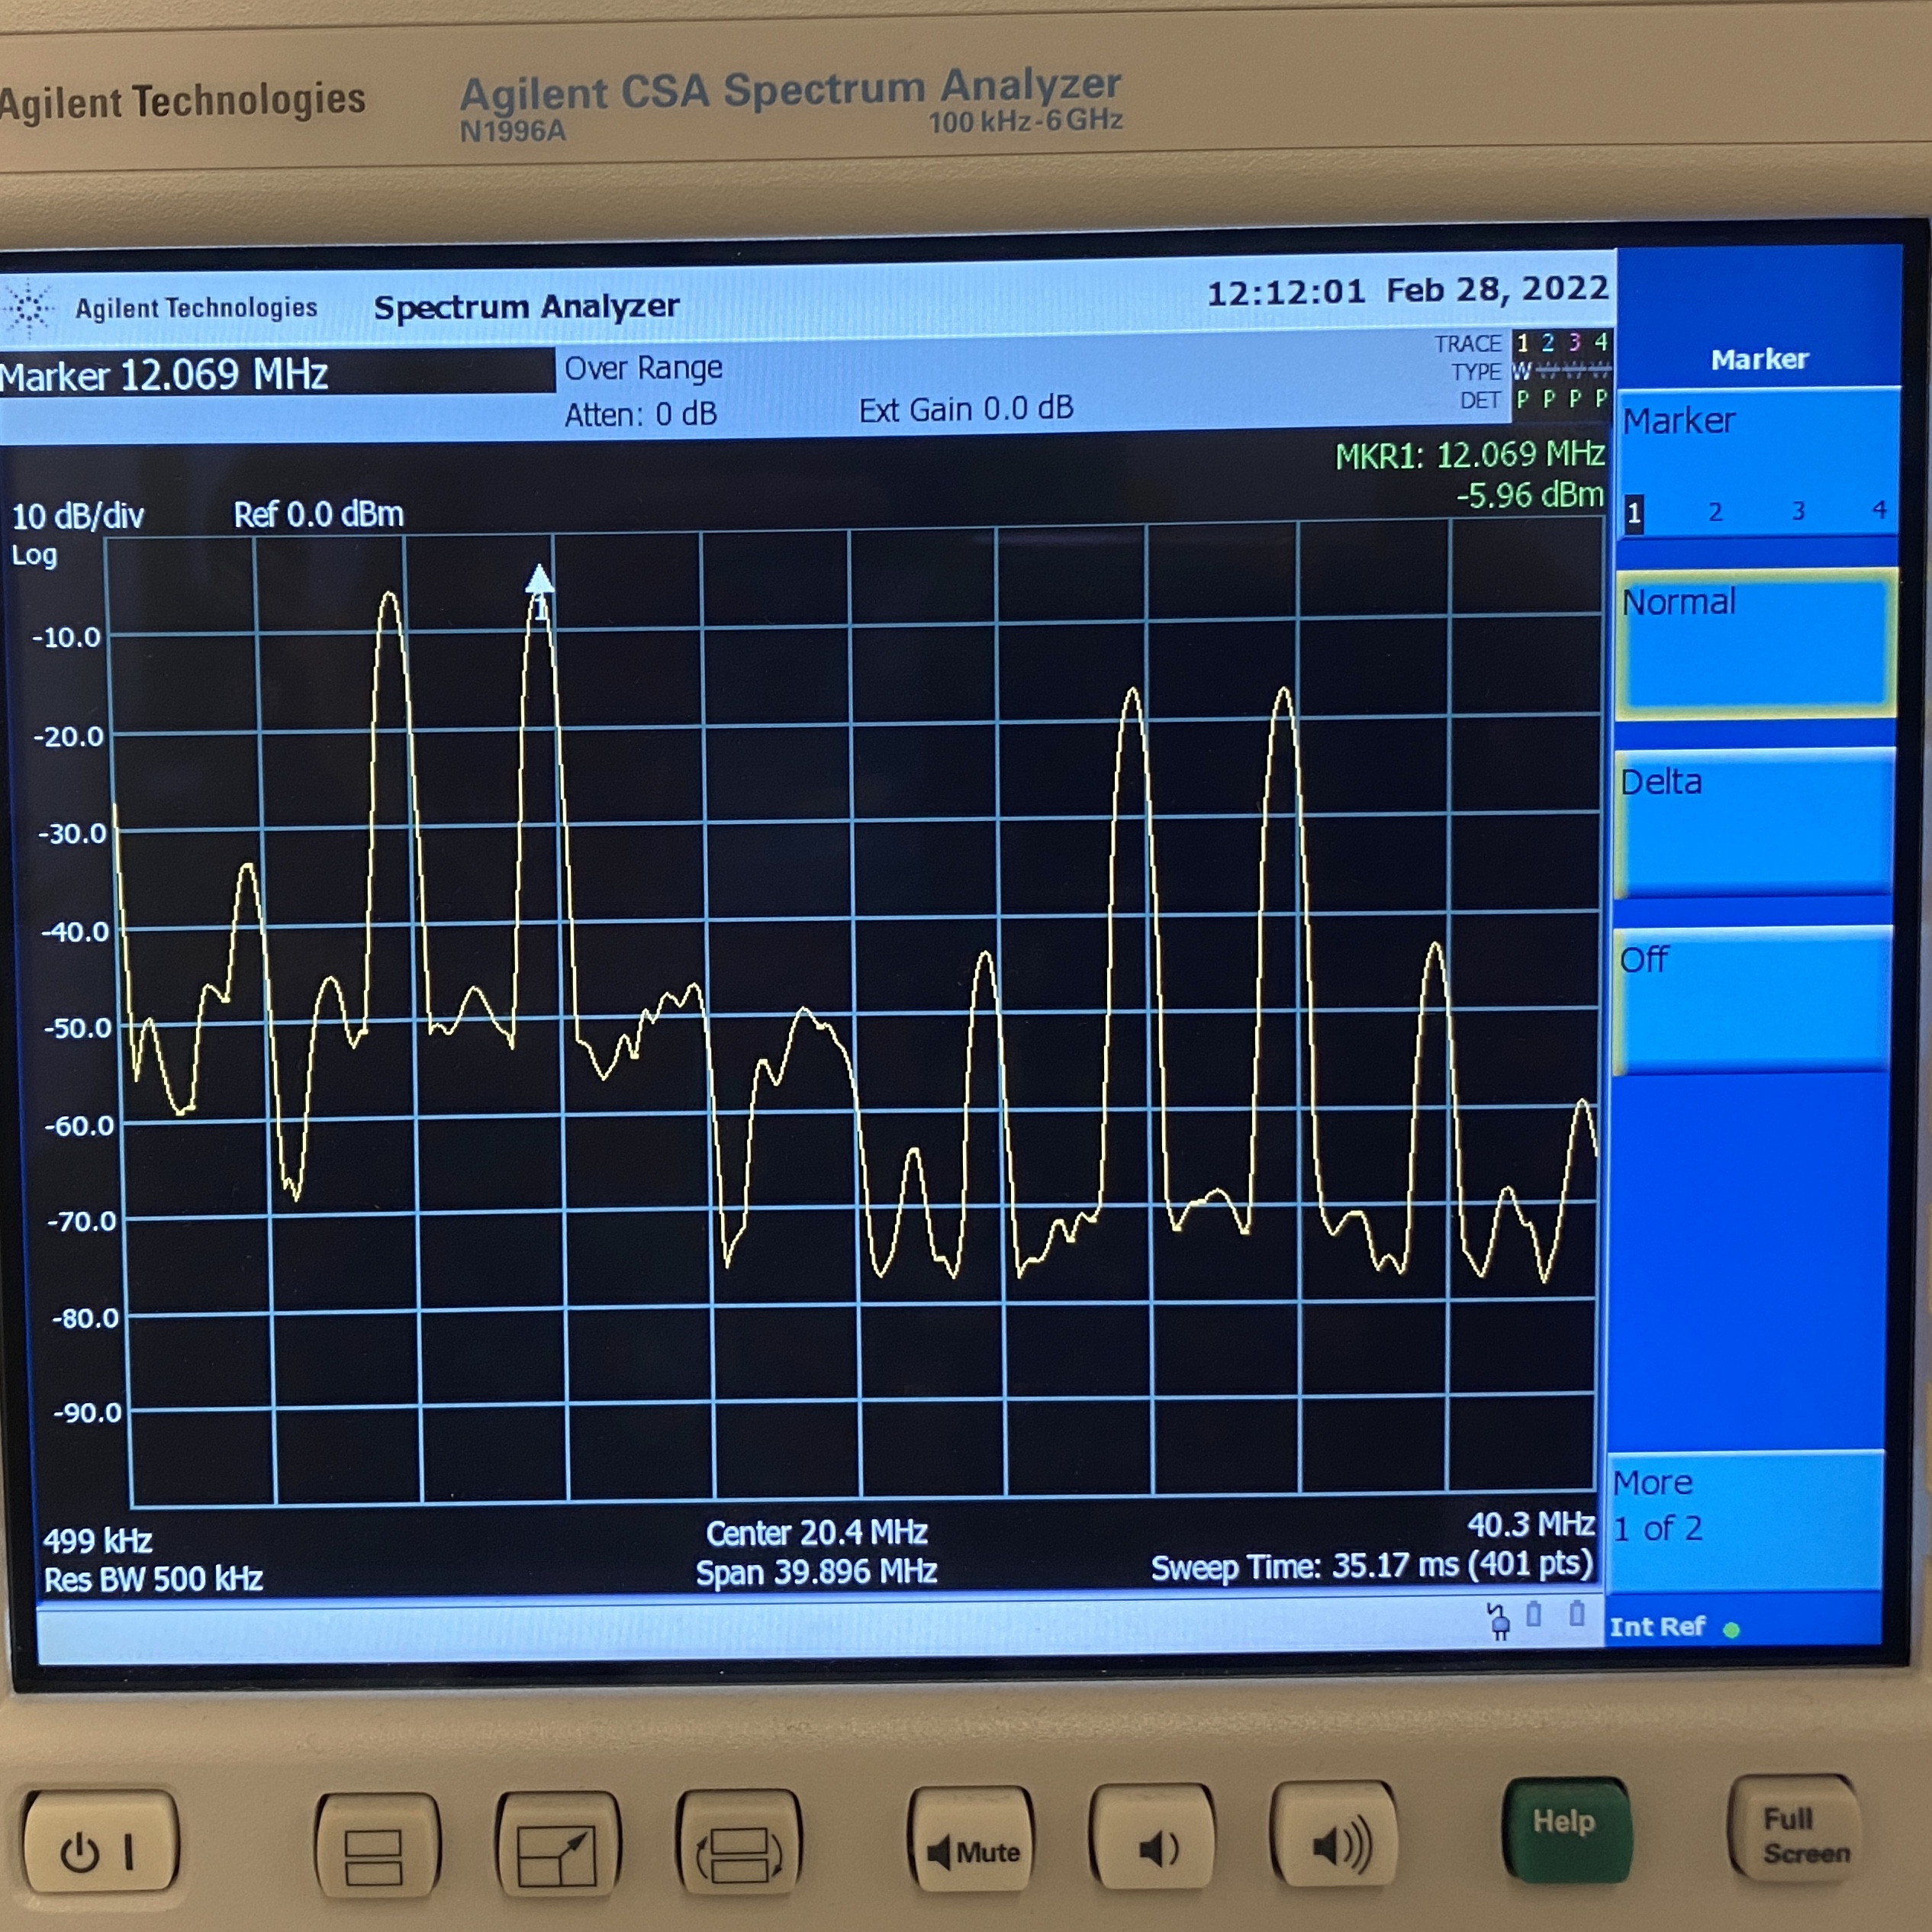
\includegraphics[width=2.5in]{fifth}%
\label{fig_third_case}}
\caption{Increasing the amplitude of LO increases the gain as well as the noise. In (a), the amplitude is $0.5\,\text{V}_{pp}$, while in (b), it is $3\,\text{V}_{pp}$}
\label{fig_sim}
\end{figure*}

\begin{table}
\renewcommand{\arraystretch}{2.2}
\begin{center}
\caption{Effect of Changing Amplitude of LO or RF}
\label{tab1}
\begin{tabular}{c c c}
\hline
\bfseries Amplitude & \bfseries Gain & \bfseries Noise\\
\hline
$\uparrow$ & $\uparrow$ & $\uparrow$\\
\hline
$\downarrow$ & $\downarrow$ & $\downarrow$\\
\hline
\end{tabular}
\end{center}
\end{table}

It is assumed that this relation will cease to hold at a certain point. But this exercise is left to the reader.

\section{Conclusion}

In this lab, we built a complex passive electronic component called a mixer. Our particular mixer utilized a transistor ring, and thus is dubbed a ``MOSFET mixer.''

Using our mixer, we were able to explore the way that signals can be added and subtracted together to get an output waveform with a new frequency.

Lastly, we discovered the amplitude-gain-noise relation. An increase in the amplitude of either input signal results in both more gain and more noise in the output signal.

\section*{Acknowledgments}
Special thanks to my lab partners Devorah and Marc for all their help and support. They have lent several of their figures to match the data which I collected in my lab notebook. Thanks also to Yifan for inspiring me to dust off my \LaTeX skills, as well as helping with several of the Tikz schematics. Finally, thanks to Joanna and Steve for their endless patience in my quest to learn electronics.

%{\appendices
%\section*{Proof of the First Zonklar Equation}
%Appendix one text goes here.
% You can choose not to have a title for an appendix if you want by leaving the argument blank
%\section*{Proof of the Second Zonklar Equation}
%Appendix two text goes here.}


% \begin{thebibliography}{1}
% \bibliographystyle{IEEEtran}

% \bibitem{ref1}
% {\it{Mathematics Into Type}}. American Mathematical Society. [Online]. Available: https://www.ams.org/arc/styleguide/mit-2.pdf

% \end{thebibliography}

\end{document}


